\documentclass[12pt,a4paper]{article}

\usepackage{epcc}
\usepackage{graphics}

\usepackage{listings}
\usepackage{xcolor}

\definecolor{codegreen}{rgb}{0,0.6,0}
\definecolor{codegray}{rgb}{0.5,0.5,0.5}
\definecolor{codepurple}{rgb}{0.58,0,0.82}
\definecolor{backcolour}{rgb}{0.95,0.95,0.92}

\lstdefinestyle{mystyle}{
    backgroundcolor=\color{backcolour},   
    commentstyle=\color{codegreen},
    keywordstyle=\color{magenta},
    numberstyle=\tiny\color{codegray},
    stringstyle=\color{codepurple},
    basicstyle=\ttfamily\footnotesize,
    breakatwhitespace=false,         
    breaklines=true,                 
    captionpos=b,                    
    keepspaces=true,                 
    numbers=left,                    
    numbersep=5pt,                  
    showspaces=false,                
    showstringspaces=false,
    showtabs=false,                  
    tabsize=2
}

\lstset{style=mystyle}


% This example file shows how a thesis can be laid out using Latex. It
% does not use any special local features so should be portable to other
% places.
%
% To produce myfile.pdf from myfile.tex type:
% 
% pdflatex myfile
%
% Note that pdflatex expects all included figures to be in PDF too. See
% the includegraphics command below.


% This document contains many cross-references and forward references,
% eg in constructing a table of contents, so Latex may need to be run
% twice to get all the references correct. If you need to run Latex twice
% you may get the warning:
% 
% LaTeX Warning: Label(s) may have changed. Rerun to get cross-references right


\begin{document}

% \title{Programming Skills: Profiling and Performance Coursework}
% \author{Rachel Dance}
% \date{\today}

% \makeEPCCtitle

% \thispagestyle{empty}

% \newpage

% \pagenumbering{roman}

% \tableofcontents

% \lstlistoflistings

% \newpage

% \section*{Acknowledgements}

% This template is a slightly modified version of the one developed by
% Prof. Charles Duncan for MSc students in the Dept. of Meteorology. His
% acknowledgement follows:

% {\em This template has been produced with help from many former students who
% have shown different ways of doing things. Please make suggestions for
% further improvements.}

\newpage
\pagenumbering{arabic}

\section{Introduction}

The objective of this work is to profile, and assess the performance of the code 'percolate'. Full details of this code are contained in the briefing document provided for this coursework, and a brief outline is given here. 
The objective of this C code is to find a continuous path of empty cells through a grid. The basic steps are to create and initiate a square grid of cells, where each is randomly assigned to be empty or full according to some density. To count and identify clusters of empty cells, the code assigns a unique integer value to all cells regarded as empty. It then loops over the grid many times, replacing the value of the empty cells with the maximum of its four neighbouring cell values in each loop, eventually reaching convergence where all cell values no longer change and a cluster is identified. Finally, it determines whether any cluster touches both the top and bottom boundaries. If this is the case, then the problem is said to 'percolate' as there is a continuous path of empty cells from top to bottom.

Section \ref{sec:method} gives a summary of key assumptions and methodologies employed when carrying out the analysis in Section \ref{sec:results_analysis}. In Section \ref{sec:initial-results}, the effect of the grid dimension (-{\em l} ) on the code performance is shown, so that it may serve as a benchmark and provide information on the parameter space to be used in subsequent sections. In Section \ref{sec:line_profiling} line by line profiling of the code was then carried out to ascertain hotspots for future optimisation. Overheads of the gprof profiler have been estimated in Section \ref{sec:overheads}.
In Section \ref{sec:optimisation_flags} performance of the code for the grid dimensions identified in Section \ref{sec:initial-results} is assessed by application of the available compiler flags, and then this is compared to benchmarks to measure the speedup. The most effective of these flags is used in Section \ref{sec:enhancements_by_o2} where the relationship between runtime and grid dimension is re-assessed and compared to Section \ref{sec:initial-results}.

\section{Experimental Method}\label{sec:method}

This code has several inputs, one of which is the grid dimension {\em l}, i.e. if $l=200$, the code will initiate the problem on a $200\times200$ grid. Profiling of the code in this work was carried out using the GNU gprof compiler \cite{ref:GNUgprof}. The code was compiled in all cases by 'gcc' \cite{ref:gcc}.

The code has several input variables, which are documented in the code 'README' file. For clarity, only the input grid dimension {\em l} was varied here. The values of  the random seed, density and maximum number of clusters are kept at 1564, 0.3 and 400 respectively.

In this work, only the grid dimension {\em l} is varied, and the code profile at values of {\em l} is interrogated, and the  performance is analysed using optimisation flags. 
Increasing the size of the grid has two effects. Firstly, that there are more cells in the system as a whole and so the code has more iterations to complete, and second, as a result of this there are then more changes in the system before the solution converges. Therefore by increasing the grid size, we are seeing a convolution of both of these effects. This ultimately means that not only does the simulation take longer due to there being more cells, but that each complete loop over the grid will take longer as there are more changes to these. Therefore we do not expect that an increase in the grid size will result in a linear increase in total time taken. We would expect this to take a similar form to $l^n$.

To analyse performance, standard gcc optimisation flags are used \cite{ref:flags}, and the code is run once again, using the same compiler and grid sizes, with one optimisation flag applied, and these are compared to those without optimisation. To reduce the chance of errors in compilation and execution, running the code was automated wherever possible.

\subsection{Automation}\label{automation}

\paragraph{For Varying grid size:}
Initially the code was compiled using a bash script, {\em build.sh} with all default values and no optimisations included. Only the -pg flag was included to enable profiling. Bash scripting was further used to perform each run of the code in precisely the same way in 'run\_pipeline.sh' (Listing 2).
\begin{lstlisting}[language = bash, caption="run\_pipeline.sh" to execute percolate in the same way for varying grid sizes.]
#!/bin/bash
names='200 500 1000 1500 2000 2500 3000 3500'
for name in $names
do
echo $name
./percolate -l $name
gprof -l percolate > ../results/grids/gprofresults_$name.dat
done
echo All done
\end{lstlisting}

A simple makefile (Listing 2) was also used to clean up the system afterwards to make sure that when a new build is carried out, that there is no interference from pre-existing files.

\begin{lstlisting}[language = bash, caption="Makefile" to clean out executable files and object files between builds]
.PHONY: clean
clean:
      	rm -I *.dat *.pgm *.o percolate *.out
\end{lstlisting}

\paragraph{For varying compiler flags:} 
To vary compiler flags, the directory is cleaned and re-built with differing flags for each build. The following bash script was used to clean, build, run and write results to a file for each flag. \begin{lstlisting}[language = bash, caption=build.sh to vary compiler flags and produce results files.]

names='-O0 -O1 -O2 -O3 -Os -Ofast'

for name in $names
do
echo Running for $name
rm -f *.o percolate
gcc -g -c arralloc.c uni.c percolate.c $name
gcc -g -o percolate arralloc.o uni.o percolate.o -lm $name
(time ./percolate -l 2500) > ../results/flags/flag_2500_$name.dat 2>&1
done
echo All done
\end{lstlisting}
The directory is cleaned of object files and previous versions of percolate, and gcc is used to re-build the file with the appropriate flags. 
To measure the time taken, the {\em time} method (Line 10) has been used to produce overall time. It was found in the initial stages of this work that optimisation flags interfere with the profiling in gprof. For flags up to '-O2', the compiler will  disable some of its optimisation if it also finds the '-pg' flag, but for optimisation levels at '-O3' or greater, then this is not the case \cite{ref:flags}, so gprof is not combined with optimisation here. This provoked the move to a more simplistic timing of the overall code performance using only the 'time' method. This produces a 'real', 'user' and 'sys' time. In this study, the 'real' time is used as this represents the absolute time used by the code, and 'sys' is the the time taken by system overheads such as opening files or other operations which can be excluded.

\subsection{Reproduciblity}\label{reproducibility}

In order to ensure that the results obtained are reproducible, and also to abide by computer usage protocols, all results were assigned to a node within Cirrus \cite{ref:cirrus} as opposed to the login node. The login node on the Cirrus machine is in demand to different levels depending on user traffic, and as such different levels of computational effort are available to jobs submitted to this node. Therefore, submitting to a separate node which does not host user traffic, will mean that a uniform amount of resource is available for code runs, leading to more stable results. This machine and this work uses the Slurm software to schedule batch jobs, more details can be found in \cite{ref:cirrus}. 


\section{Results and Analysis}\label{sec:results_analysis}

\subsection{Initial results}\label{sec:initial-results}

To gauge the parameter space taken by this problem, the code was initially run with all default values. No optimisation flags were used.
\begin{figure}[h]
\begin{center}
\resizebox{0.90\hsize}{!}{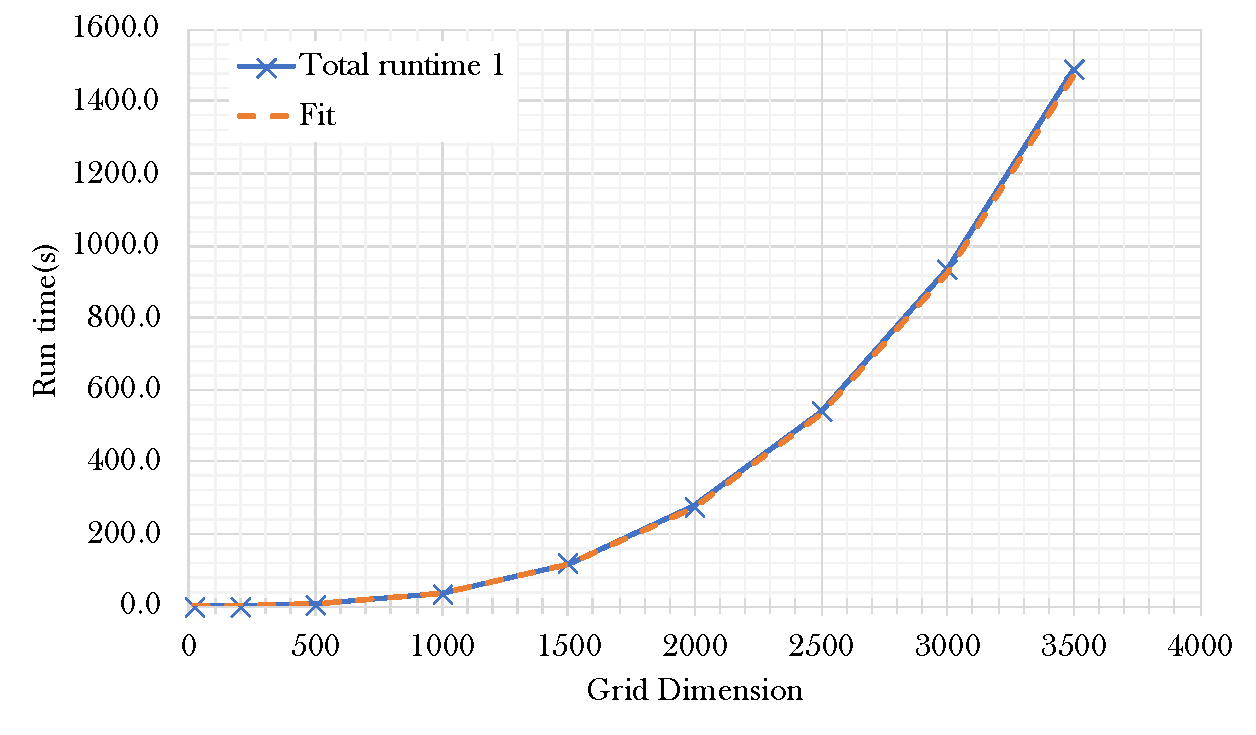
\includegraphics{figures/fig_initial_grid_times.pdf}}
\caption{Runtime with all default parameters and no optimisation with increasing grid dimension {\em l}.}
\label{fig:fig_initial_grid_times}
\end{center}
\end{figure}
In Figure~\ref{fig:fig_initial_grid_times}, it can be seen clearly that as mentioned in Section \ref{sec:method} this does not follow a linear trend as one might expect. The fit function shown on the graph, is given in Equation \ref{fit_func}.
\begin{equation}\label{fit_func}
y = 3.50\times10^{-8}{\em l}^{3} 
\end{equation}

Figure \ref{fig:fig_initial_grid_times} shows  that this is a close fit to the experimental data, and that the runtime (y) is a function of ${\em l}^3$. This part of the study was not extended beyond {\em l} = 3500 as the runtime of the experiment became prohibitively large. By this equation, a grid size of {\em l} = 5000 would take approximately 1 hour 10 minutes, and to increase an order of magnitude to 10000 would take upwards of 9 hours. Without the ability to go up in orders of magnitude, it was not deemed that any further insight was likely to be gained by increasing to {\em l} = 5000. These results show that the runtime for {\em l=2500} is not prohibitively long with no optimisation, and a short test (not documented here) shows it is also able to provide a non-zero runtime when fully optimised. 

The error associated with the results given in Figure \ref{fig:fig_initial_grid_times}, given by the standard error of the three trials carried out, was of the order of 0.2\% and as such is not shown by error bars.

\subsection{Estimation of Profiling Overheads}\label{sec:overheads}

In order to make a simple estimate of the overheads of the gprof profiling, the code was run for a grid dimension {\em l} = 2500. The {\em time} method was used as in Listing 4 where gprof was not used. The run time with the gprof flags was 541.5s, compared to a run time of 539.9s without the same flags, yielding a change in runtime of 1.7s (or 0.03\%). Upon repetition of this result, a standard error of 0.2\% was also found.

\subsection{Line by line profile}\label{sec:line_profiling}

The output of gprof when used with the {\em -l} option was output to files, and the flat profile part of the gprof output reveals the time spent by the code in each individual line. From this, it was seen consistently across all grid dimensions tested that the code spends upwards of 99\% of its time in lines 148 to 161.
The profiling reported here reported percentages greater than 100\% (for example, 100.18\% for {\em l} = 500 which by definition, is not a valid result. However, as all other lines on the flat profile are reading 'no time accumulated', which is interpreted to mean that the code is spending a vanishingly small amount of time in other lines. To optimise this code, these lines should be targeted as they form almost all of the run time.

To break this down further, at three points in the analysis, {\em l} = 200, 1500, 3000 the time spent on these lines was analysed more closely to ascertain that the time spent on these lines varies with the size of the input grid. Figure \ref{fig:fig_time_on_lines} shows the line by line results from the flat profile output from gprof. 

\begin{figure}[h]
\begin{center}
\resizebox{0.90\hsize}{!}{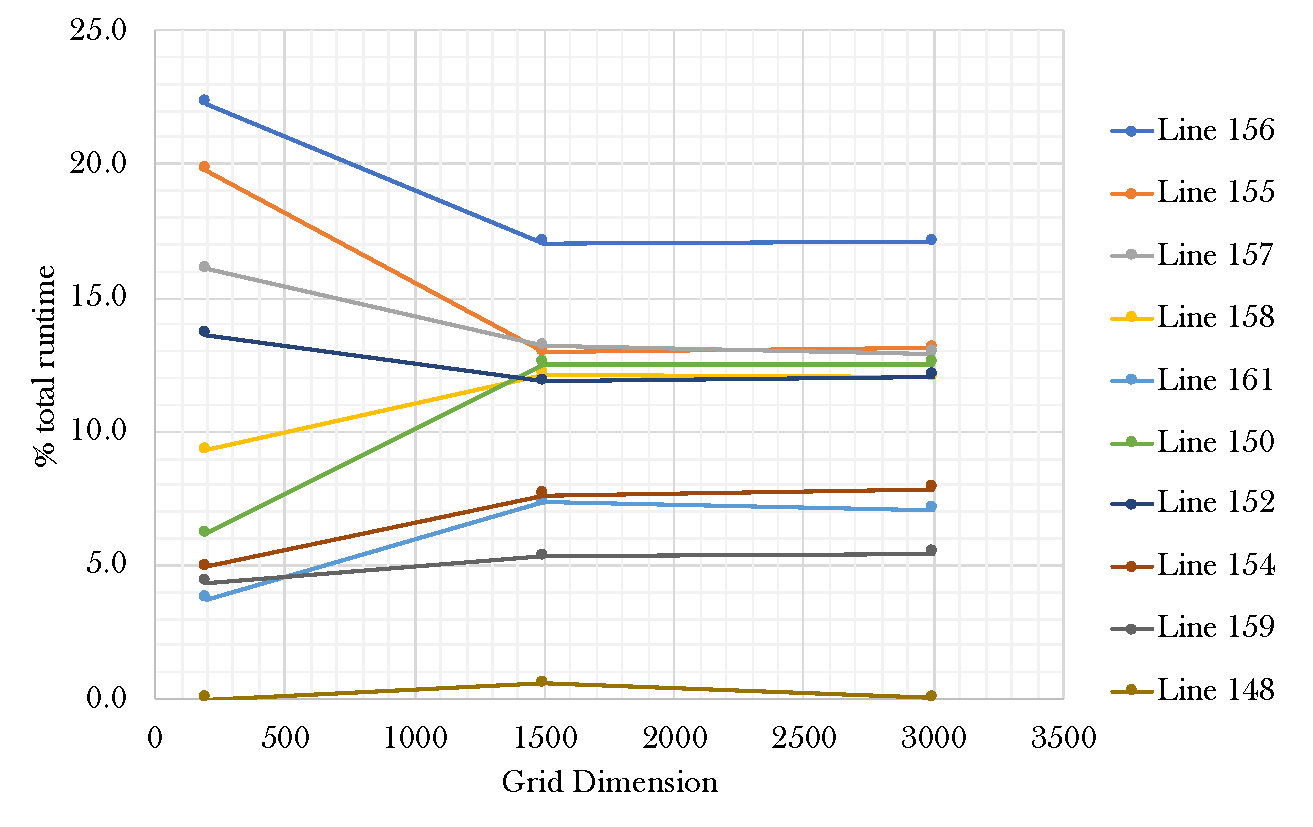
\includegraphics{figures/fig_time_on_lines.pdf}}
\caption{Time spent on lines 148-161 for grid dimensions {\em l} = 200, 1500 and 3000.}
\label{fig:fig_time_on_lines}
\end{center}
\end{figure}

These three increments in grid dimension were chosen to show the extent of the parameter space used, without producing an incomprehensible graph. Straight lines between points do not represent data, but are left in place to guide the reader on the link between data sets. Figure \ref{fig:fig_time_on_lines} shows that for a grid size of {\em l} = 200, there is some variation in the proportions of time spent on the lines studied, but there is very little difference between {\em l} = 1500 and {\em l} = 3000. For a grid size {\em l} = 200, the run time is so fast that is is possible that the profiler itself is not able to measure line timings, but this was a repeatable result and occurs consistently. The error once again on these values (not shown as error bars) is of the order of less than 1\%.

Another interesting observation from this profiling exercise was the amount of time per call to the random function. This code calls the {\em 'random\_uniform'} method on source code line 118, to decide whether each cell is empty or full when the grid is initialised. It is therefore expected to be called ${\em l}^2$ times for any grid dimension {\em l}. Upon closer inspection it was found that the time taken per call was not uniform, and is dependent on the number of grid cells in the problem.
\begin{table}[h]
\begin{center}
\begin{tabular}{|c|c|c|c|c|}
\hline
{\bf Grid dimension} & {\bf #Number of calls} & {\bf Time for one call (s)} & {\bf Total time (s)}\\
\hline
200 & 4.00E+04 & 6.76E-06 & 0.27\\
1500 & 2.25E+06 & 6.68E-09 & 0.02\\
3000 & 9.00E+06 & 5.01E-09 & 0.02\\
\hline
\end{tabular}
\end{center}
\caption{Analysis of time spent on random number assignment.}
\label{randint_calltime}
\end{table}
Table \ref{randint_calltime} shows significant variation in the time used by the random function each time it was called, depending on the grid dimension used. Not that times given are absolute. In real terms, neither a microsecond or nanosecond are significant periods of time, and the time spent by the code in all three scenarios is small. However, there is no discernible reason that there should be {\em any} change in time per usage of the random function when the grid dimension increases, and this discrepancy becomes visible when the code is called many times.

\subsection{Performance enhancements using compiler flags}\label{sec:optimisation_flags}

From Section \ref{sec:initial-results}, a grid size of {\em l} = 2500 was chosen for more studying the effect of compiler flags. 
\begin{table}[h]
\begin{center}
\begin{tabular}{|l|c|l|c|l|}
\hline
{\bf Flag} & {\bf Real (l=2500} & {\bf Real (l=2500} \\
\hline
O0 & 539.599 & 34.881 \\
O1 & 237.067 & 15.472\\
O2 & 204.878 & 13.377 \\
O3 & 205.275 & 13.406\\
Os & 216.89 & 14.107\\
Ofast & 215.277 & 13.105\\
\hline
\end{tabular}
\end{center}
\caption{Total time (\%) spent in lines 148-161 for grid dimension {\em l} = 2500.}
\label{flag_table_2500}
\end{table}

\begin{figure}[h]
\begin{center}
\resizebox{0.90\hsize}{!}{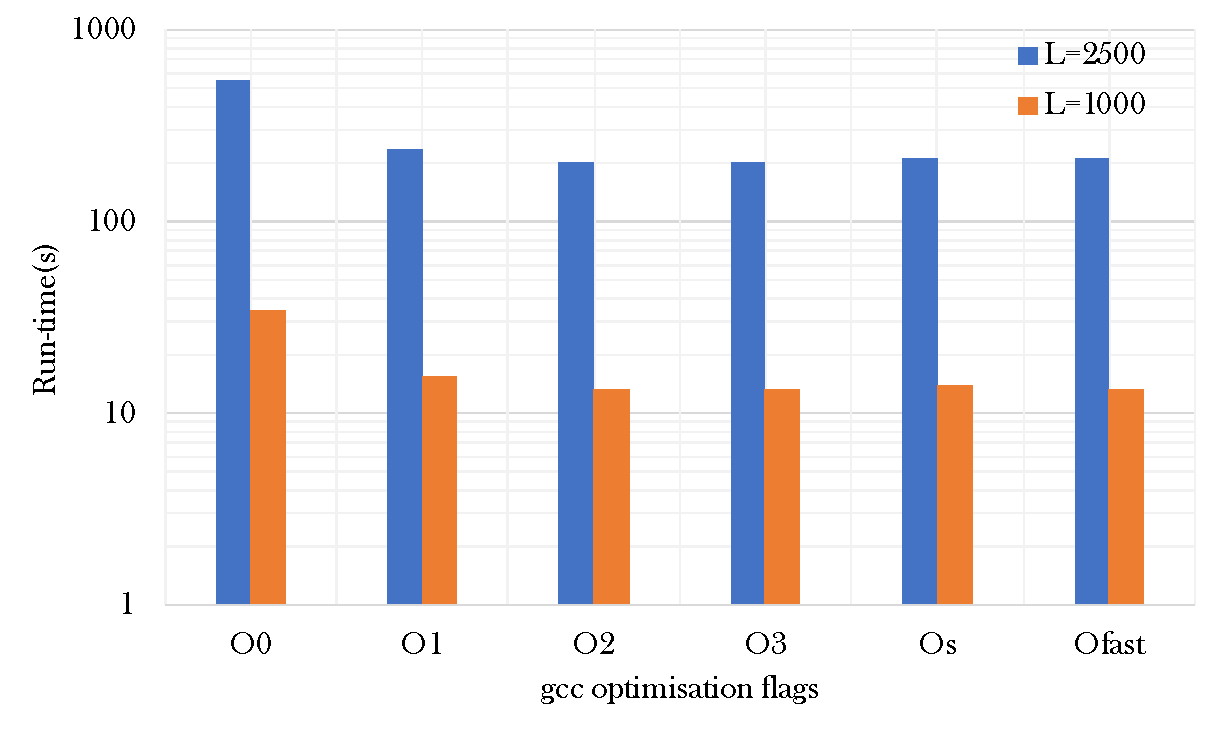
\includegraphics{figures/fig_gcc_flags.pdf}}
\caption{Runtime results for use with gcc compiler optimisation flags. Note the logarithmic scale in  runtime.}
\label{fig:fig_gcc_flags}
\end{center}
\end{figure}

Figure \ref{fig:fig_gcc_flags} and Table \ref{fig:fig_gcc_flags} show that the most significant reduction in runtime is achieved between the use of no optmisation at all (flag O0) and the use of the lowest level of optimisation (flag O1). This is consistently seen to provide 40-50\% reductions. The reductions beyond this in both cases of {\em l} = 1000,2500 is minimal. It is also seen that the compiler optmisation flag '-Os' produces a slight increase in run time in both cases - this is not visible in Figure \ref{fig:fig_gcc_flags}, but can be seen on inspection of table \ref{flag_table_2500}. As it provides the most reduce runtime for the minimal interference of optimisation, the flag '-O2' is used in the final performance part of this work.

\subsection{Effect of optimisation on runtime}\label{sec:enhancements_by_o2}

In order to assess the effect of the compiler on total runtime, the code was run once again as it was in Section \ref{sec:initial-results} with the same grid dimensions but including the compiler flag '-O2'. In order to make a meaningful comparison, the code was run with no profiling, and no optimisation and the 'time' method was used to calculate runtime, as described in Listing 4. This revealed that there was no change when compared to the inclusion of profiling in agreement with Section \ref{sec:overheads} and thus the results from Section \ref{sec:initial-results} are comparable. 

Figure \ref{fig:fig_speedup} shows the comparison of these results to Section \ref{sec:initial-results}. The -O2 flag was chosen as stated in Section \ref{sec:optimisation_flags}.
\begin{figure}[h]
\begin{center}
\resizebox{0.90\hsize}{!}{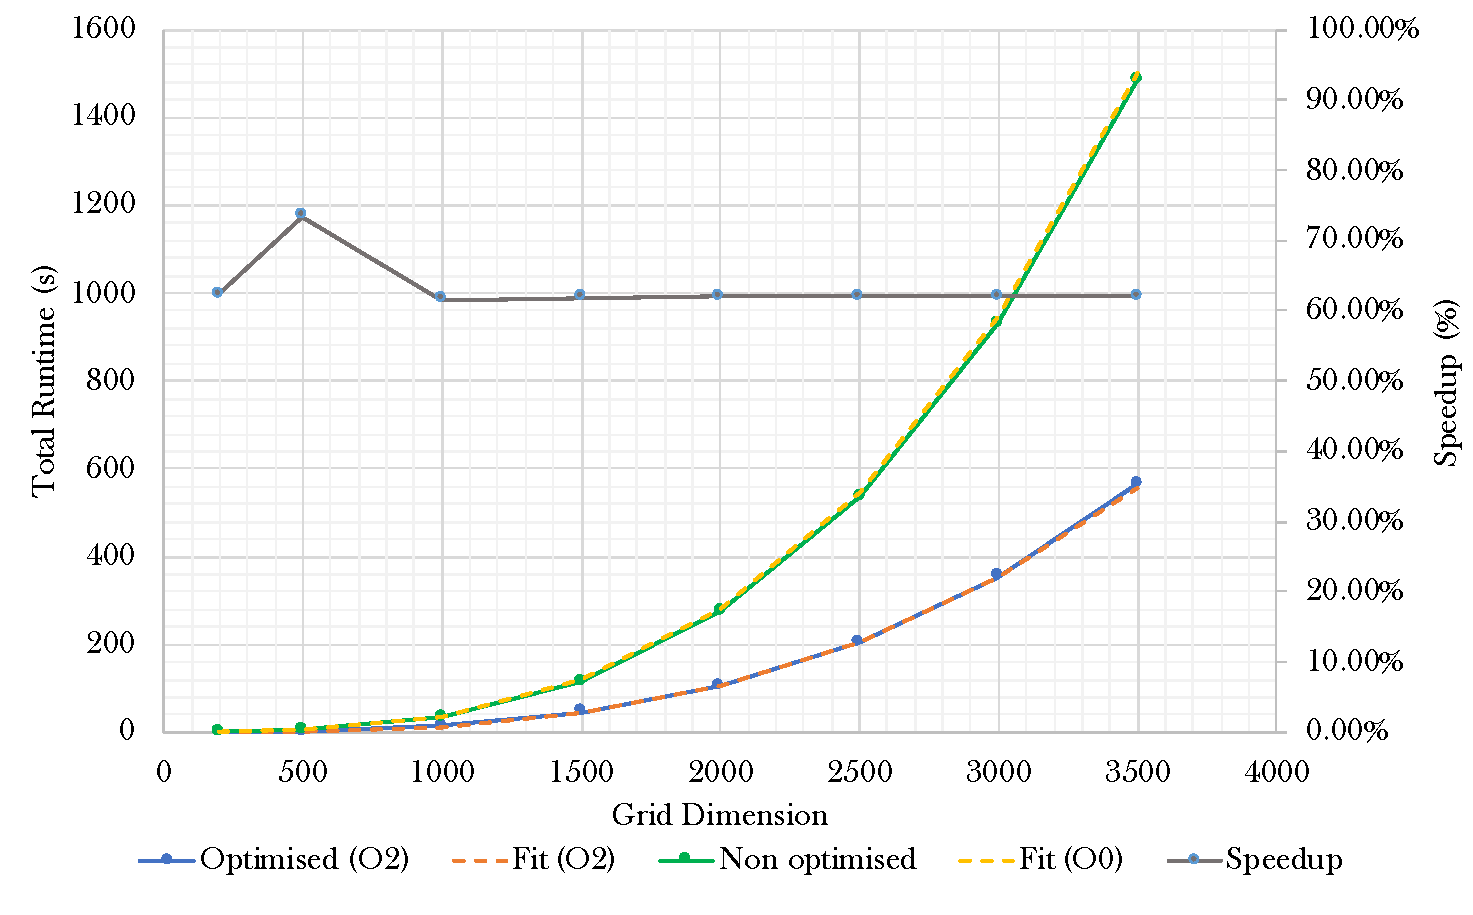
\includegraphics{figures/fig_speedup.pdf}}
\caption{Runtime results for use with gcc compiler optimisation flags.}
\label{fig:fig_speedup}
\end{center}
\end{figure}
As was done in Section \ref{sec:initial-results}, a fit function was also identified (Equation \ref{fit_func_2}), and was also found this to be of the same form as Equation \ref{fit_func}. 
\begin{equation}\label{fit_func_2}
y = 1.50\times10^{-8}{\em l}^{3} 
\end{equation}
Therefore we can see that the change in runtime remains a function of $l^3$, but the coefficient has halved meaning that the curve is shallower as can be clearly seen, and over the parameter space used here, the runtime is reduced in reduced by 62\%. For the cases where {\em l} = 500 the results show an increased speedup of 70\%. 

\section{Conclusions}

Initial runs of the code with no optimisation showed that the runtime increases as a function of $l^3$. In order to assess the errors on this value due to the usage of the gprof profiler, the additional time spent solely due to the compiler was found to be $<1\%$. 
Line by line profiling using gprof indicated that approximately 100\% of the runtime was spent working on line 148-162, which is the loop in the that reads and updates the grid to find and identify the clusters. Analysis shows that the code spends minimal time (an immeasurably small amount in fact) on other aspects. Therefore we can conclude here that any optimisation should be spent in these lines. changes in other areas will only produce minimal gains in performance.

One of the key ways to improve performance was to use the compiler flags provided as part of the gcc. Use of each compiler was applied to a grid dimension {\em l} = 2500, and total runtime showed that the '-O2' flag provided the biggest improvement.
Finally, in order to assess the speedup achieved by the addition of this optimisation flag, it was compared to a set of runs with the same grid dimension as used in Section \ref{sec:initial-results}. This analysis found that the code runtime remains a function of $l^3$, but with the coefficient reduced by half. 

An additional observation was made in Section \ref{sec:line_profiling}, that the time taken per call of the {\em'random\_uniform'} method on line 118, also changed with the grid size, but no trend was identified.

\subsection{Future Work}

Further investigation to complement this work could be carried out to determine whether the use of optimisers changes the proportion of time spent on each individual line of code.
This could not be done here as the gprof profiler was found to be altered by the use of the optimisation. 
Attempts could also be made to optimise the lines identified here as a hotspot, namely lines 148-161 of the source code. The runtime of the rest of the code could also be identified by removing the main loop from the code into external function calls. As gprof is a function analysing profiler, and this code exists as one continuous function as it is small, the information it produces can be limited, so alternative profilers could be used.


\begin{thebibliography}{100}

\bibitem{ref:GNUgprof}Documentation:{\text{ https://ftp.gnu.org/old-gnu/Manuals/gprof-2.9.1/html\_mono/gprof.html}} Accessed 20/11/2020.

\bibitem{ref:gcc} GNU gcc compiler manual: {\em https://gcc.gnu.org/} Accessed 20/11/2020.

\bibitem{ref:flags} GNU Documentation, Optimiser flags: { https://gcc.gnu.org/onlinedocs/gcc/Optimize-Options.html} Accessed 20/11/2020.

\bibitem{ref:cirrus} Cirrus 1.2 documentation. [online] Available at: https://cirrus.readthedocs.io/en/master/ [Accessed 24 Nov. 2020].

\end{thebibliography}

\end{document}

